\subsection{Retrospective molecular illustrations}
Figure~\ref{fig:cases} presents retrospectively selected successful examples from both tasks in scaffold split 17. These illustrations explain the prediction outputs; they are not additional independent validation. Task~1 examples are assay-defined analogue pairs; Task~2 examples are individual molecules evaluated by their departure from the training-only assay-pair median. Each scatter shows the full held-out cohort for the displayed pair. The highlighted compounds illustrate retained or reversed SAR and small or large molecular sensitivity, while the complete cohorts also expose prediction errors.

For Task~1, the CHEMBL288 analogue pair retains its assay-A ordering: the observed and predicted A-oriented assay-B gaps are $+1.620$ and $+1.621$ pIC$_{50}$, with predicted SAR-loss probability 0.024. The CHEMBL237 pair reverses its ordering; its observed and predicted oriented gaps are $-1.000$ and $-0.952$ pIC$_{50}$, with predicted loss probability 0.981. The corresponding pair cohorts contain 29 and 38 held-out comparisons. Structures and measured assay potencies are shown in the figure.

For Task~2, the two ROCK2 compounds have observed sensitivities of 0.291 and 0.678 pIC$_{50}$, with predictions of 0.285 and 0.731; cohort MAE is 0.106 over 13 molecules. For estrogen receptor $\beta$, the observed values are 0.326 and 1.300, and predictions are 0.457 and 1.335; cohort MAE is 0.337 over 16 molecules. For ALDH1A1, observed values are 0.372 and 0.707, and predictions are 0.440 and 0.680; cohort MAE is 0.268 over 20 molecules. AUROC values for these complete cohorts are 0.825, 0.844 and 0.835, respectively. Raw assay potencies and compound identifiers are reported in Table~\ref{tab:caseprovenance}.

\begin{figure}[p]
\centering
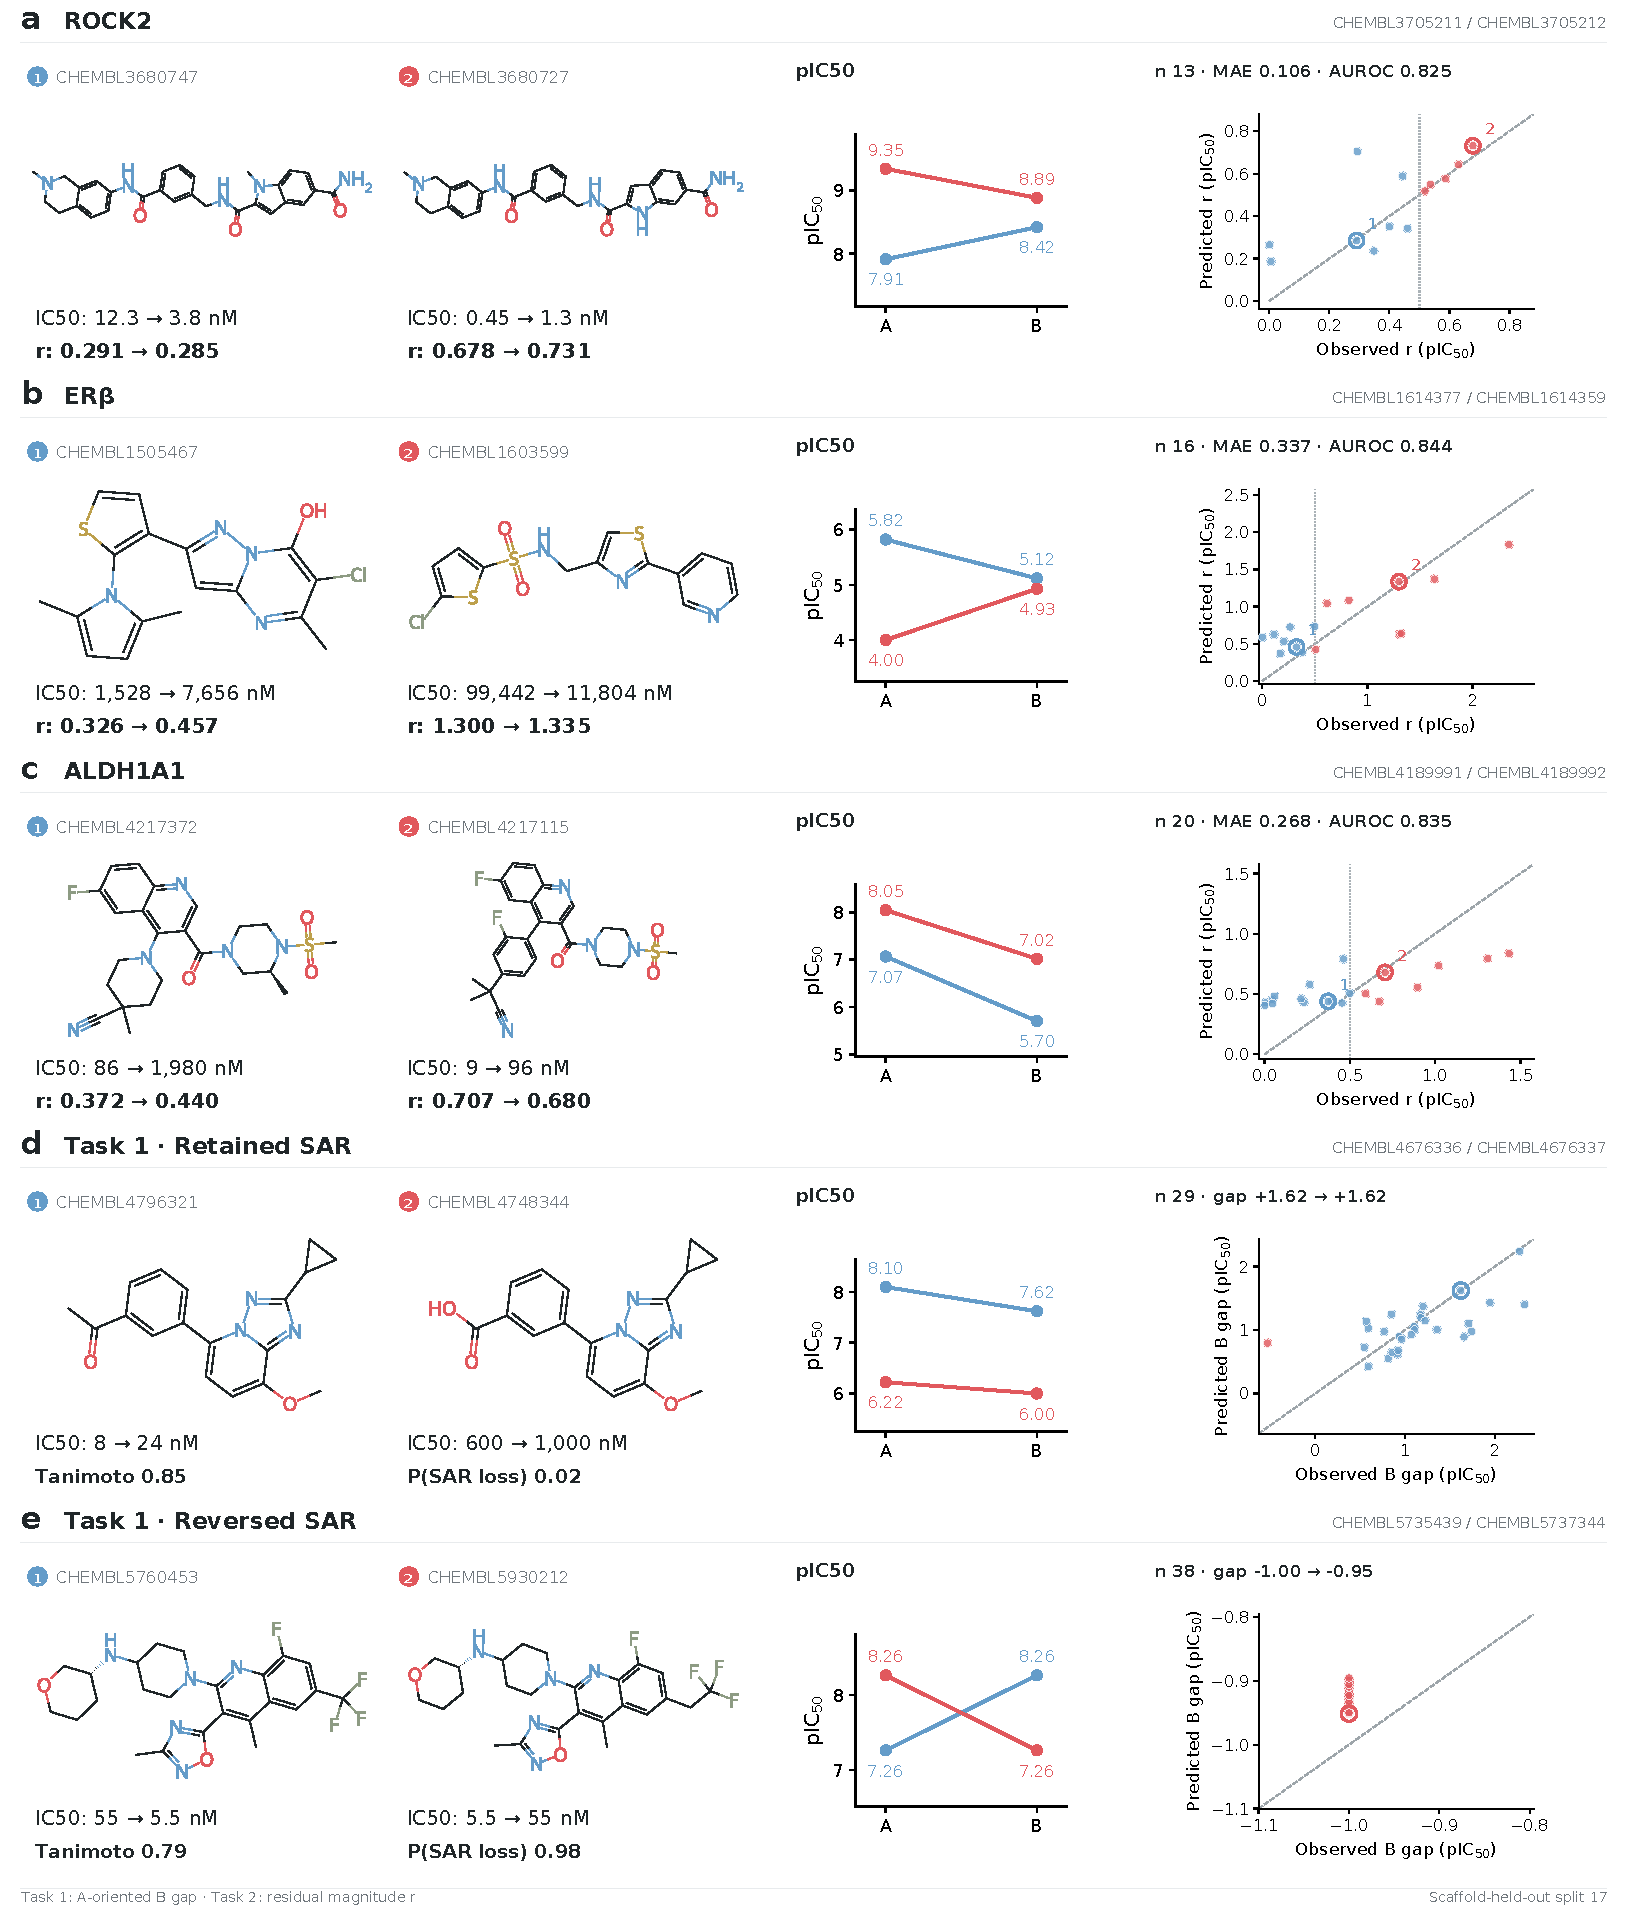
\includegraphics[width=0.98\textwidth,height=0.88\textheight,keepaspectratio]{figure4_casebook.pdf}
\caption{Retrospectively selected molecular illustrations in scaffold split 17. (a--c) Task~2: activity-linked structures, measured assay-A/B potencies, and complete assay-pair test-cohort sensitivity predictions for ROCK2, ER$\beta$ and ALDH1A1. Numbered compounds match the highlighted scatter points. (d,e) Task~1: two matched analogue pairs with retained and reversed SAR, their measured potency tracks, and complete selected-pair test-cohort predictions. B gaps are oriented by the assay-A ordering; the ring highlights the displayed analogue comparison.}
\label{fig:cases}
\end{figure}

\begin{table}[htbp]
\centering
\caption{Measured potencies and held-out residual predictions for the displayed Task~2 compounds. Error is absolute difference in pIC$_{50}$ units; compound identifiers link to source structures.}
\label{tab:caseprovenance}
\small
\begin{tabular}{@{}llrrrrr@{}}
\toprule
Target & Compound & A (nM) & B (nM) & Obs. $r$ & Pred. $r$ & Error \\
\midrule
ROCK2 & CHEMBL3680747 & 12.3 & 3.8 & 0.291 & 0.285 & 0.006 \\
ROCK2 & CHEMBL3680727 & 0.45 & 1.3 & 0.678 & 0.731 & 0.053 \\
ER $\beta$ & CHEMBL1505467 & 1.53e+03 & 7.66e+03 & 0.326 & 0.457 & 0.131 \\
ER $\beta$ & CHEMBL1603599 & 9.94e+04 & 1.18e+04 & 1.300 & 1.335 & 0.036 \\
ALDH1A1 & CHEMBL4217372 & 86 & 1.98e+03 & 0.372 & 0.440 & 0.067 \\
ALDH1A1 & CHEMBL4217115 & 9 & 96 & 0.707 & 0.680 & 0.027 \\
\bottomrule
\end{tabular}
\end{table}
